%%
%% Author: shoupu_wan
%% 7/14/18
%%

\chapter{Variational Method for Software Development} \label{ch:variational}
Given a fairly complex project, it is hardly ever the case to arrive at the optimal design and
implementation at the first attempt, even for experienced senior engineers.

`quantum tunneling' effect: not every step leads to better code quality or bringing your closer
to the target solution.
Beneficial attempts may come from purposeful exploration in the opposite direction.

Below is my testimony when I was designing and implementing a \code{ProtobufVisitor} module.
\begin{quotation}
    How I came to a better design by introducing a method called isEmpty()

    When handling the visitation of repeated fields of protobuf during a design of visitor pattern,
    my brained was twisted several rounds.

    A repeated field is a field where a list of elements may be recorded in one place.
    In general, the essential information regarding repeated fields are the size of the list, the
    positional indexes, and the elements themselves.
    On the one hand, the repeated field as a list may be of interest, even elements that
    are simply empty messages.
    On the other, the elements in the list are often more important.
    But under certain circumstances, not all of the info is desirable.
    For example when counting for the presence of fields, we need just a Boolean per field.
    Any more information than would be wasteful and burdensome.

    But my visitor pattern is designed for generic use.
    I am designing it for the most detail-oriented applications as well as the minimalists'
    applications.
    How may I make my base classes most useful as to doing most all the weight lifting work while
    conveniently leaving the flexibility of choices to client?

    I tried with more complex design of the element classes.
    I also tried with more complex algorithm to
    avoid visiting empty messages.
    All the effort was to no avail.

    Finally and desparately, I approached the problem from another perspective---as the Chinese
    old saying has it ``Treat head for headache and foot for foot pain.''
    Now that the problem is with the specific use case of field presence tally,
    I put a special logic to count the
    presence of the total elements in the repeated field.
    Then I put a recursive algorithm to remove
    the ancestors of nodes where count = 0.
    It worked!
    Of course only for this specific case.

    Then I abstracted the concept to represent the count = 0 condition as \code{isEmpty()} and put
    this in the base class.
    Now my visitor pattern design and implementation is more flexible and generic.

    It allowed client code to specify if repeated field significance is of importance while lift
    away the burden of removing the unimportant parts from the overall result.
    All by overriding the \code{isEmpty()} method.

    A good design takes away much of the weight lifting things that's common and known while leaving
    the variable parts and use case specifics to client to make a call.
    The balance may be subtle and
    the solution may be scarce, but rest assured that there is always an 'aha' design awaiting
    for discovery somewhere.
    It clicks within your brain when you found it.
\end{quotation}

\section{Principle of Variational Method}\label{sec:principleOfVariationalMethod}

This is an account of my experience of implementing visitor pattern for protobuf translation and
iteration for the purpose of schema mapping.

I have to admit by now that I'm no genius.
I'm quite clumsy, witless, and ordinary.
My way of working is not ingenious, either.
Nevertheless I can produce something of quality with long-time contemplation,
perseverance, divine inspiration, obsessive insistence, a good sense of judgement, and hard work.

This method is what I called `variational method', and it proves an effective tool to help
me asymptotically approach the desirable result.
The method itself is pretty mechanical.
But it takes several characters out of the developer to execute it successfully.

I'm going to explain the method in details in the following sections.

\subsection{Prerequisite---developer characters}\label{subsec:prerequisiteDeveloperCharacters}

Yes, the prerequisite lies in developer characters instead of knowledge or skill sets.

Though the method itself is mundane, one needs to have certain
characters to successfully carry it out.

\subsubsection{Hard work}

With any idea of any quality, you need to put it to experiment.
Start with an implementation and see its result.
No idea should go untested.
That requires hard work.
Long-time thinking.
You cannot work for long without thinking.
Take a walk away from your desk to help you concentrate.
More often than not, ideas will be like rain pour over you while you are walking after a long
struggling work at no avail.

\subsubsection{Perseverance}

You can be passionate but that state won't last without perseverance.
Many times i observed myself become impatient, desperate, depressed in that order.
But I kept going on anyway.
At various stages, I was almost convinced that there is no way out or I cannot find a way out.
But due to a trace of belief and perseverance, I didn't give up.
For example, I am not happy with a design of template interface at some point.
My gut feeling tells me that there got to be a better way to arrange the types, algorithms, interfaces such that
the template has minimum implementation required.
I believe it's a suboptimal design.
But I've been trying for several times with no hope of seeing this process converging anywhere.

\subsubsection{Divine inspiration}

I am a Christian and I derive my strength from my Lord.

I can hardly forget that throughout the process of the hair-pulling project, I prayed, a lot.
I take breaks by prayers and Bible study.
It's not for profit that I turn to our Lord Jesus.
I just enjoy being around of Him.
God is my Shepherd I shall not want.
His presence comforts me.
I depend on Gods inspiration.
And He never let me down.
When I walk or on train, ideas pour on me like rain drops.
My urge to hurry back to try them is almost unrestrainable.
For fear of forgetting, I often hastily wrote them down in short-hands before they dry out on me!

\subsubsection{A sense of good judgement}

Good judgement is a character that controls engagement and/or disengagement of your resource.
It tells me when to keep looking for options and when to start try out;
when to keep working out a plausible solution and when to give it up.

This also tells me when to settle and accept what I've got.
Quality of work never come easy.
It's a perpetual process of improvement.
It's like the learning curves which is often nonlinear with steep and hart ramps and drooping
valleys.
Sometimes the quality of code gets stuck with no improvement for a long time.
Some times it even regresses.
On rare occasions, it improves with an excellent, serendipitous idea by a great amount.

Good judgement is like the sixth sense, an eye of your heart, that guides you through the paths of
the hardship.

Good work is like a `click'.
You can sense the imperfect.
You can `feel' the underlying problems because the discomfort is `right there'.
Your gut feeling can even measure how big the problem is.

\subsubsection{Essence of the variational method}
``After all these'', you ask, ``what is variational method of software development?''
It's bit by bit.
It's convergence oriented.
It's about deferred detail.
But foremost, variational method requires a clear goal in mind.
A goal that is specific, contained, and measurable.
`Measurability' is pretty relaxed here---as long as your gut feeling can tell if you attained it
or not, it is measurable.

With a goal in mind, and then you need a good a starting point from which may approach the goal.
There are generally two phases.

Phase one exploration

You tentatively, and shallowly experiment with various approaches.
Because it is explorational, don't try to cram in too much details.
You need hops, skips, and jumps along the line.
After a brief evaluation of multiple plausible approaches, pick one and follow through it.
If you can reach the goal with the chosen approach, congratulations, you just discovered your first
\emph{one} viable approach.
If it turns out to be dead ended or you grow bearish with it, switch to your other options.
If you truely exhausted all your options, most likely than not, you have at least one viable
approach as your starting point.
Only do not settle.

Phase two, convergence.
You narrow the solution down to a local optimum, bit by bit.
What do I mean by `bit by bit'?
Choose some steps, vary your design or implementation or both, and leverage your good judgement,
then you make a call if that variation caused improvement or regression.

In case you get stuck for too long, you can `kill' some time by nitpicking on minor flaws and
make fixes to them.
This will help clear up factors and hiding places that blind you, so in the next round you may
spot treasures just around the corner.

Go down your list of flaws, big or small, just keep improve without giving up.
Try various ways to get rid of flaws one at a time.
The strange thing is that as you make these progresses, your inner uneasiness may not decrease or
even increase sometimes.
Keep moving forward.
Don't give in until you get rid of the next flaw.
The wonderful thing is that before you reach the end of road, you often can find new ways, much
much better ways to make even bigger improvement.
This is a self-propelling process---finding defects and fix them and this will bring you to new,
bigger defects to fix.

as you strive to move forward, you find yourself closer and closer to the critical point when
with a big roar, the the inner uneasiness that has ever been in you suddenly heaves itself out of
you like a blob of cancerous cells and you are entirely relieved from all shadowy feelings.

And this proves your gut feeling of something wrong is real in the first place!

~\autoref{fig:variational-commits} please find a picture of the commit history I made during
my implementation of the visitor pattern for protobuf schema in variational approach.

\begin{figure}[htb]
    \begin{center}
        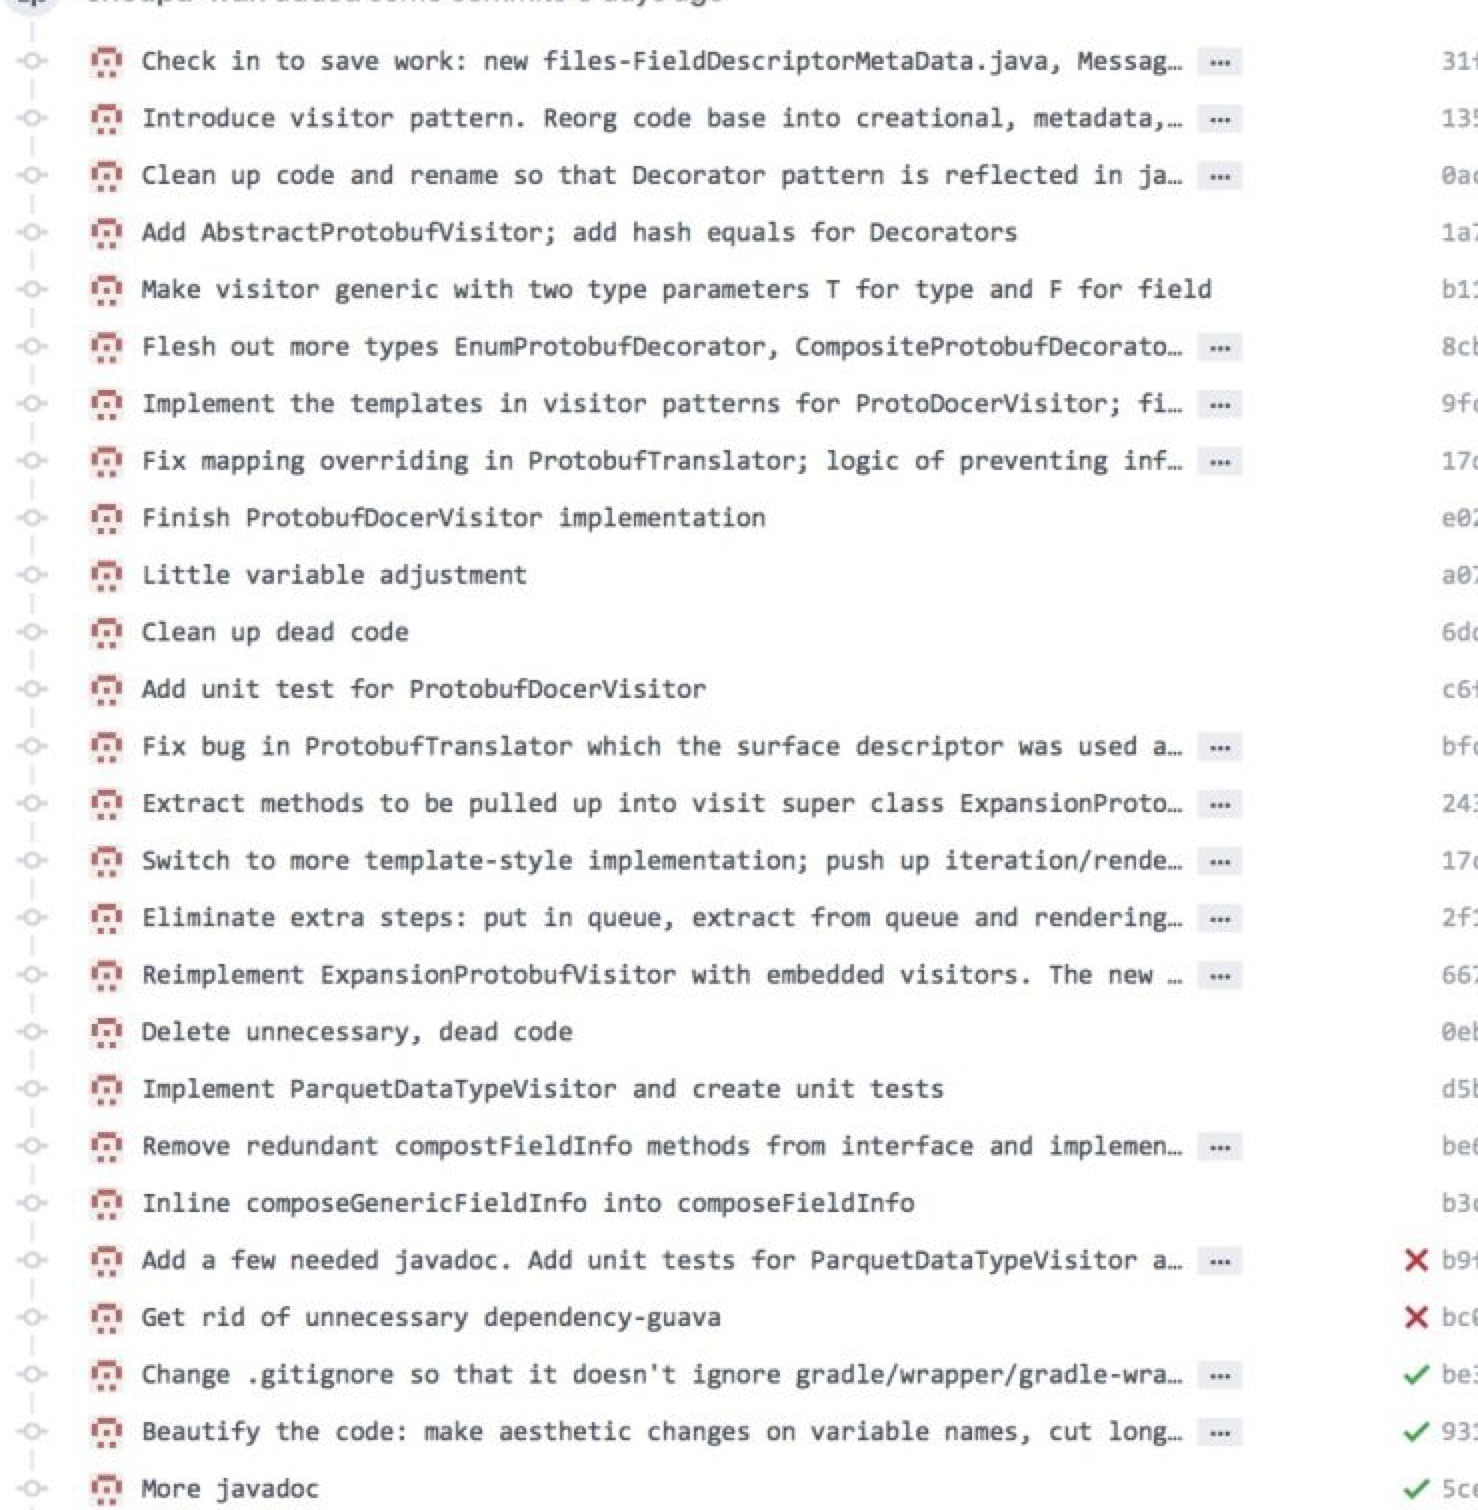
\includegraphics[height=6cm]{variational-commits.jpg}
        \caption{An example of applying variational methods to improve an implementation of protobuf
        message visitor pattern.}
        \label{fig:variational-commits}
    \end{center}
\end{figure}


\section{Case study: Find the M-th smallest element in 2D sorted matrix}

\label{Evernote:Find the M-th smallest element in 2D sorted matrix}

\section{Case study: Protobuf Descriptor}

\section{Working mode}


\section{Interactive development}

Beginning software developers often mistakenly depict the activity of software development as
linear, progressive, mechanical translation:
\begin{quote}
    Requirement $\rightarrow$ Design $\rightarrow$ Implementation $\rightarrow$ Algorithm
    $\rightarrow$ Test as shown in ~\autoref{fig:static-picture-software-dev}.
\end{quote}

\begin{figure}[htb]
    \begin{center}
        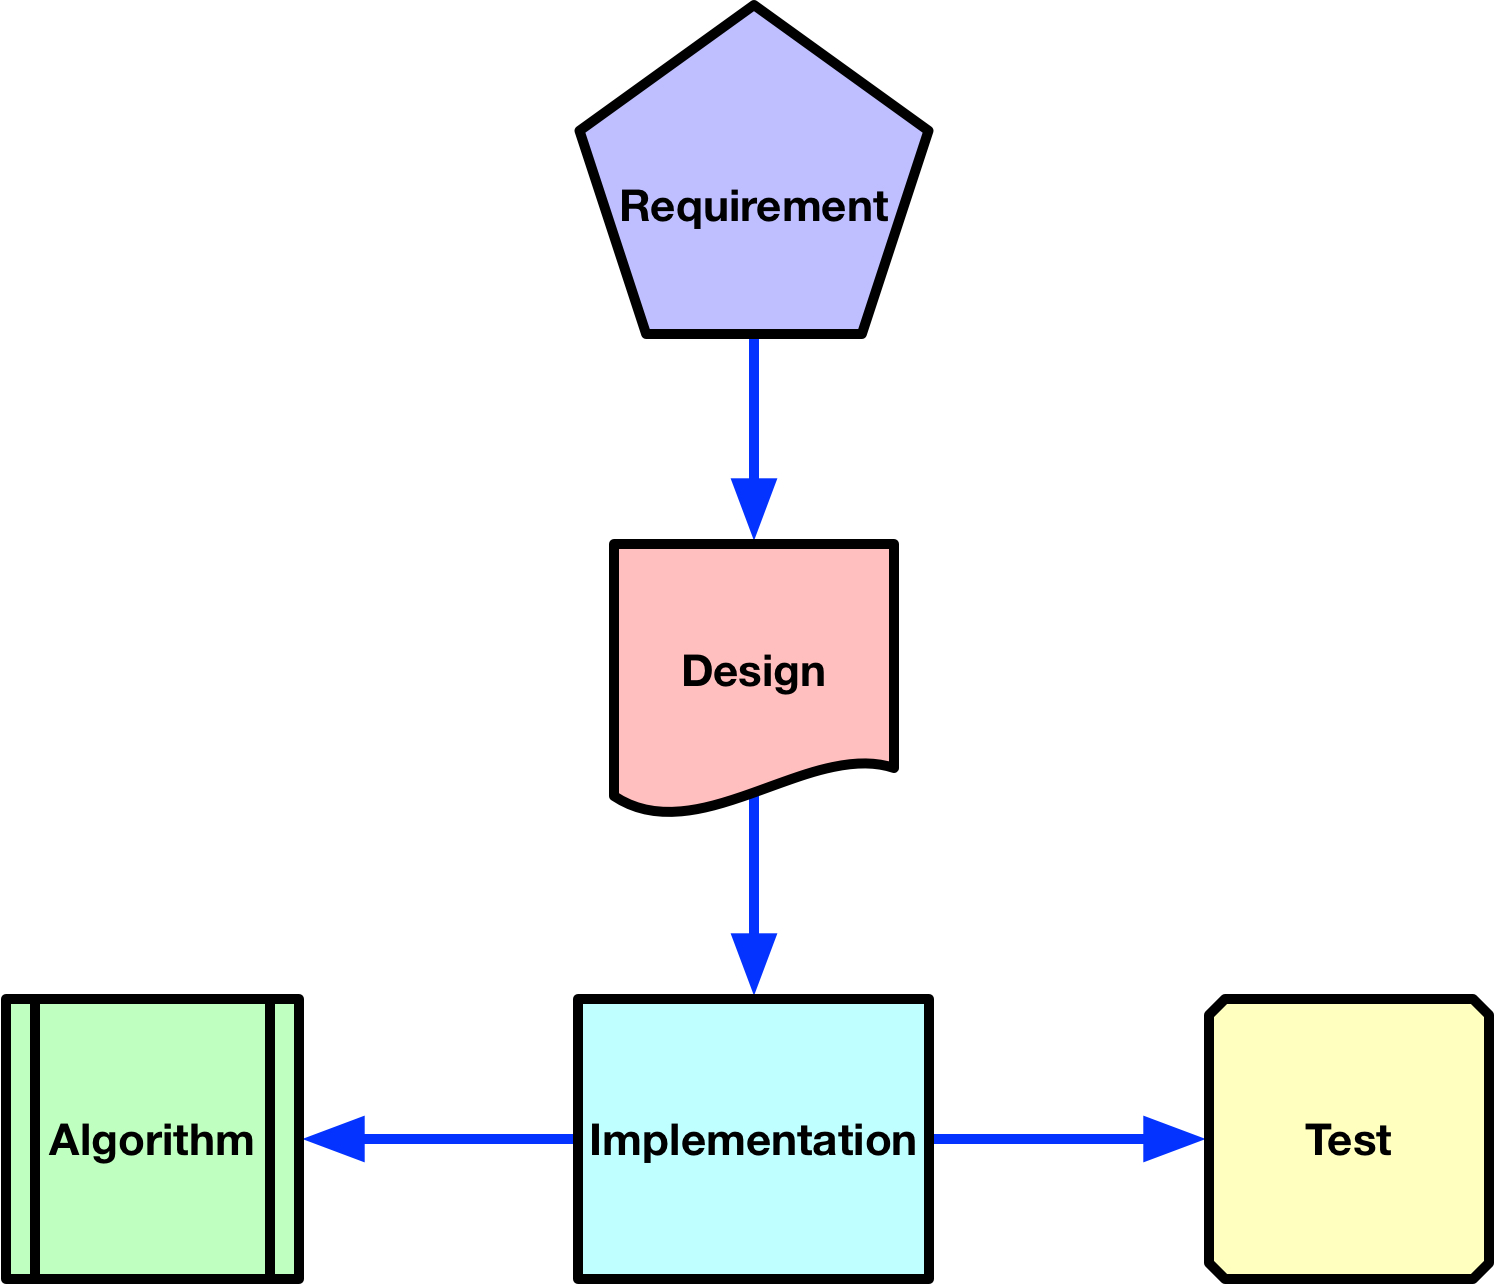
\includegraphics[height=6cm]{design-algorithm-implementation-test.jpg}
        \caption{Static picture of software development.}
        \label{fig:static-picture-software-dev}
    \end{center}
\end{figure}

If you are extremely lucky and jumped in halfway a genius team, this linear working model may be
possible.
But in reality, this is seldom the way software development works.
The reality is that software development is an involved, interactive, and entangled process.

While the main thread of the process is the forward movement, namely, from requirement, to
design, from design to implementation, \textit{etc.}, there are multiple channels for feedback
and each one of them may involves several iterations of `feedback, adjustment, feedback again, and
adjustment again $\ldots$' (see ~\autoref{fig:interactive-picture-software-dev}).

Most engineers who worked on real-world projects should have experienced some of the short
iterations between two adjacent stages, \textit{e.g.}, between test and implementation, as shown in
~\autoref{fig:interactive-picture-software-dev}.
Some experienced senior engineers may have even undergone painful iterations involving $3$
or more stages such as
\begin{quote}
    `\emph{test} $\rightarrow$ \emph{design} $\rightarrow$ \emph{implemenatation}'.
\end{quote}

While it may be a major setback to change designs after one finds out that the algorithm
to solve one of the problem is $NP$-hard, it would be much more costly if one
uncovered a flaw in the requirement at test time that jeopardize the validity of the entire system.


\begin{figure}[htb]
    \begin{center}
        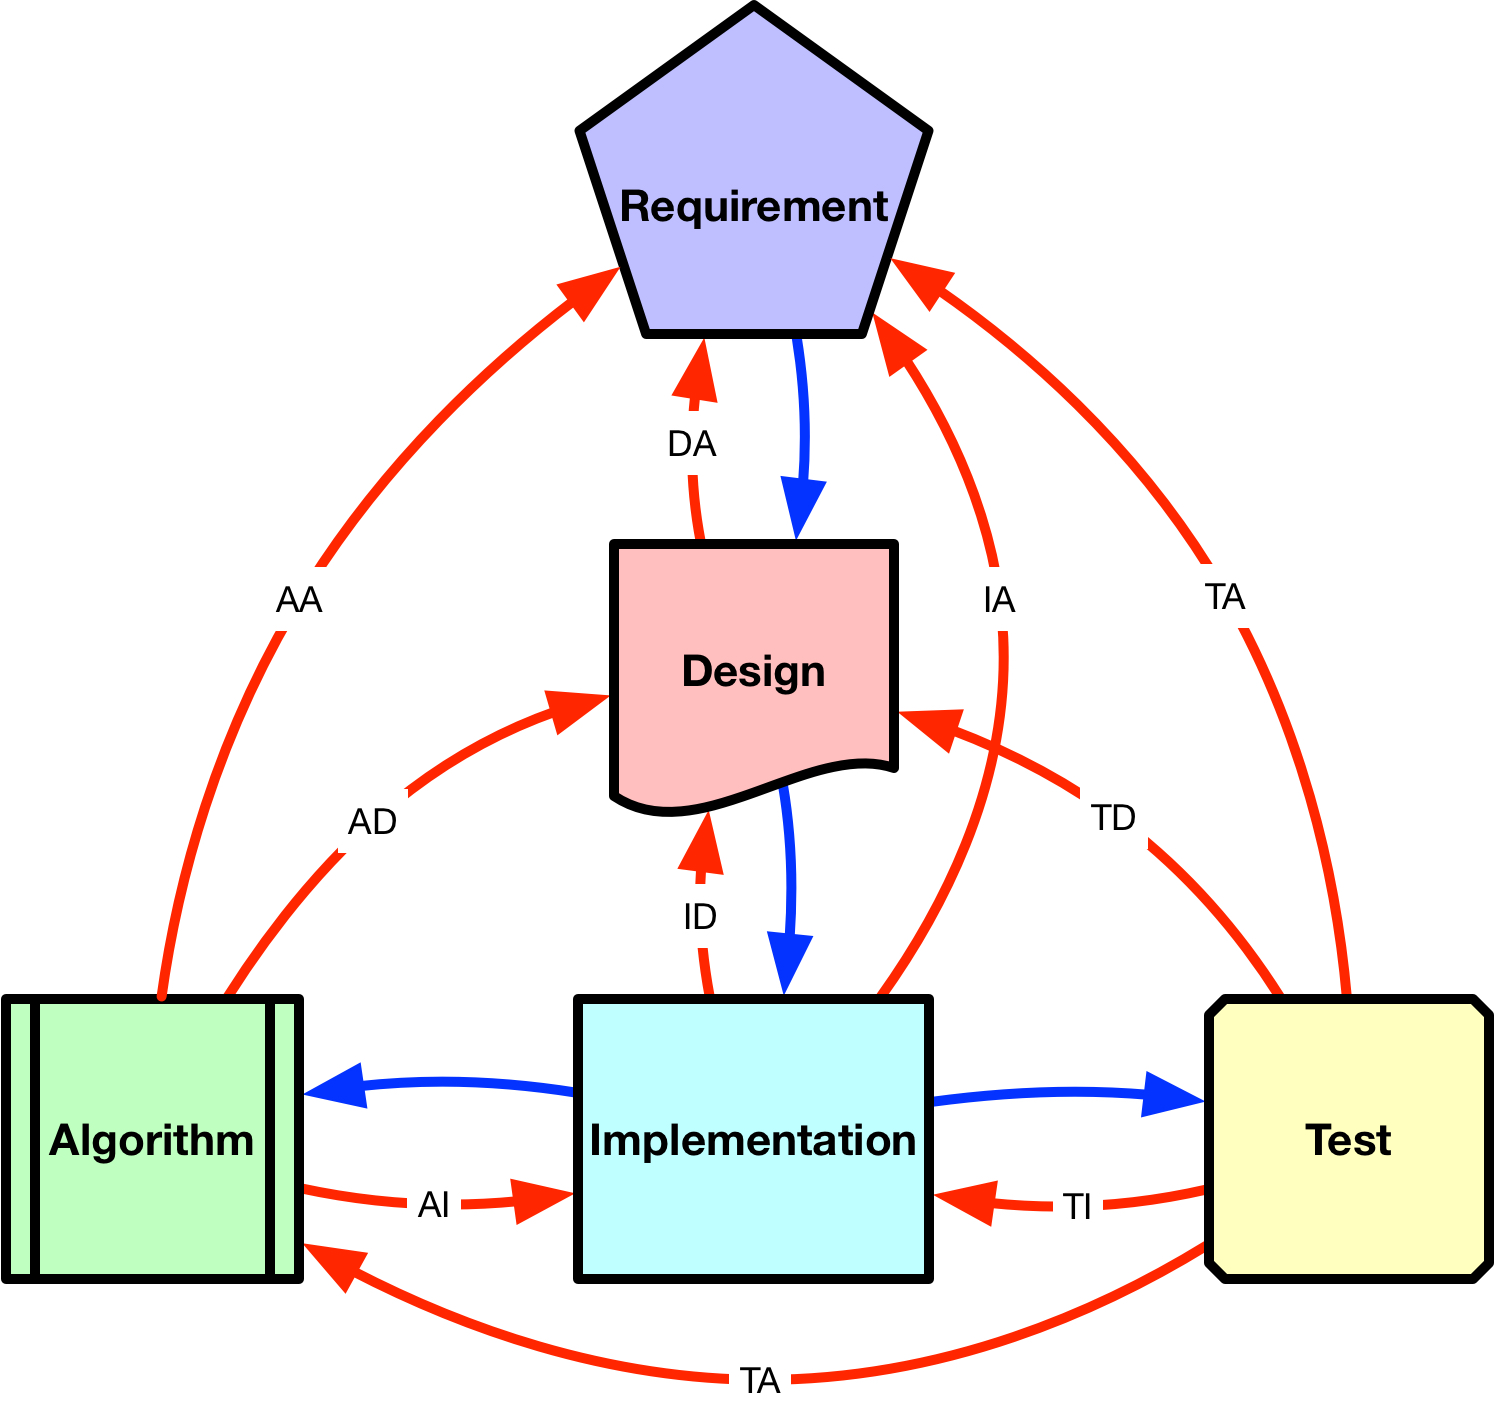
\includegraphics[height=6cm]{design-algorithm-implementation-test-fb.jpg}
        \caption{Dynamic, interactive picture of software development.
        The whole software development involves interactive and iterative feedback and improvement.
        Many things are built temporarily only to be torn down later.
        Without building them first, the final product wouldn't be possible.
        The diagram shows many such venues of feedback and, generally speaking, the longer the
        line, the costly to accommodate of the feedback venue.}
        \label{fig:interactive-picture-software-dev}
    \end{center}
\end{figure}

To summarize, software development is
\begin{itemize}
    \item It is interactive---a process with back and forth fit and retrofit.
    \item It is iterative--- with progress and setbacks that leads activities from stages to
    another stage.

    \item It is embedded---local iterations between adjacent activity stages may be nested in
    larger iterations between requirement and implementation and so on.
\end{itemize}
